\documentclass[10.5pt, twocolumn]{article}

\usepackage[english]{babel}
\usepackage{graphicx}
\usepackage{imakeidx}
\usepackage{mathrsfs, amsmath}
\usepackage{systeme}
\usepackage{array}
\usepackage[utf8]{inputenc}
\usepackage{siunitx}
\usepackage{booktabs}
\usepackage{adjustbox}
\usepackage{geometry}
\geometry{a4paper,total={150mm,225mm}}
\usepackage{makecell}
\usepackage{afterpage}
\usepackage{listings}
\usepackage{subcaption}
\usepackage[toc,page]{appendix}
\usepackage[table]{xcolor}
\usepackage{pifont} % ding symbols
\usepackage{tikz}
\usepackage{changepage}
\usepackage{multirow} % multi row in tables
\usepackage{booktabs}
\usepackage{textcomp} % registered and copyright symbol
\usepackage{lscape} % vertical instead to horizontal 
\usepackage{longtable} % for more page tables
\usepackage{eurosym}
\usepackage{lmodern}
\usepackage{amstext}
\usepackage{pdfpages} % import pdf pages
%\usepackage[hidelinks]{hyperref} % delete ugly hyperref borders of hyperlink
\usepackage{hyperref} % internal hyperlinks
\usepackage{titling} % titles
\usepackage{blindtext} % for casual texts
\usepackage{dblfloatfix} % forces image at bottom in two-column files
\usepackage{gensymb} % standard unit of measurement

\DeclareRobustCommand{\officialeuro}{%
  \ifmmode\expandafter\text\fi
  {\fontencoding{U}\fontfamily{eurosym}\selectfont e}}



\makeindex[columns=2, title=Indice alfabetico, options= -s mystyle.ist, intoc]

\newcommand*{\Scale}[2][4]{\scalebox{#1}{\ensuremath{#2}}}
\renewcommand*\contentsname{Indice}
\newcommand*\NewPage{\newpage\null\thispagestyle{empty}\newpage}
\newcommand{\Virgolette}[1]{``#1''}
\newcommand*\circled[1]{\tikz[baseline=(char.base)]{
	\node[shape=circle,draw,inner sep=2pt] (char) {#1};}}
\newcommand{\tikzcircle}[2][red,fill=red]{\tikz[baseline=-0.5ex]\draw[#1,radius=#2] (0,0) circle ;}%command for draw text circle coloured
\def\changemargin#1#2{\list{}{\rightmargin#2\leftmargin#1}\item[]}
\let\endchangemargin=\endlist
\makeatletter
\let\originalpart=\part


            
\newcolumntype{C}[1]{>{\centering\arraybackslash}p{#1}}
\newcolumntype{L}[1]{>{\arraybackslash}p{#1}}
\newcolumntype{R}[1]{>{\raggedleft}p{#1}}
\newcolumntype{G}[1]{>{\centering\arraybackslash\columncolor{gray0}}p{#1}}

\definecolor{gray0}{gray}{0.9}
\definecolor{gray1}{gray}{0.7}
\definecolor{gray2}{gray}{0.4}

\lstset{
	literate = {α}{{$\alpha$}}1 {∆}{{$\Delta$}}1 {θ}{{$\theta$}}1 {η}{{$\eta$}}1 {→}{{$\rightarrow$}}1 {∂}{{$\partial$}}1, %tutti i simboli da usare come codice
	language = Mathematica % linguaggio
}
\hypersetup{
	citebordercolor=red
}


% ----- TITLE
\title{
	\large{University of Trento}\\
	\normalsize{Master in Mechatronics Engineering}\\
	\vspace{0.2cm}
	\large{\textit{Modelling and simulation of mechatronic systems}}\\
	\vspace{0.2cm}
	\Large{\textbf{Development, analysis and optimization of the performance of an innovative driving simulator}}\\
	\vspace{0.25cm}
	\hrule
	\vspace{0.2cm}
	\large{\textbf{System requirements}}\\	% Title
	\vspace{0.2cm}
	\hrule
}
\author{A. Comoretto \and J. Losi \and S. Valentini}
\date{}
% ----- TITLE


\begin{document}
\maketitle
The objective of this project is to develop, analyze and optimize the performance of an innovative driving simulator.
A simulator is a device that enables the operator to reproduce or represent under test conditions phenomena likely to occur in actual performance.
Driving simulators are in general used both for research purposes and in the development process of a vehicle.

The simulator has to emulate the behaviour of a car like the one shown in Figure \ref{f:ReferenceSystem}.
\begin{figure}[h!]
	\centering
	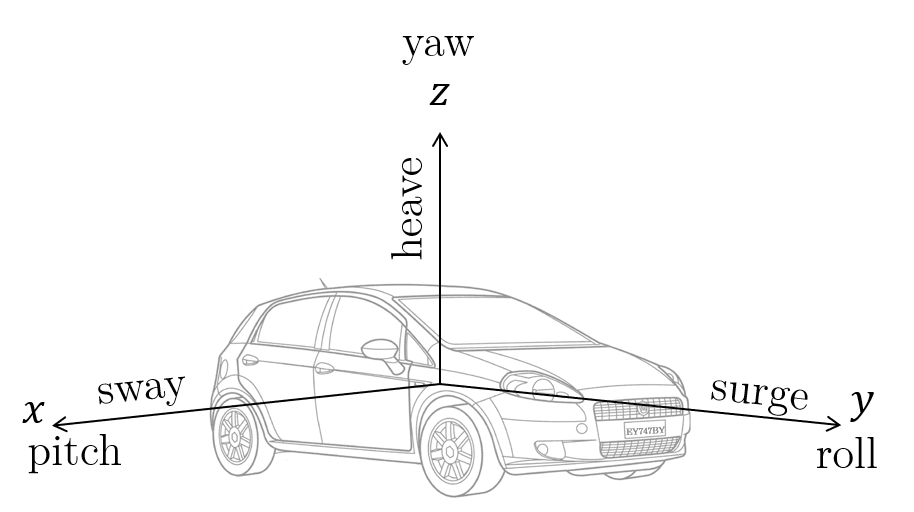
\includegraphics[width=5cm]{Images/Car_axes}
	\caption{Reference system used.}
	\label{f:ReferenceeSystem}
\end{figure}
In the first phase of the project it is relevant to impose a correct set of objective which are composed by system requirements, engineering specifications and performance indexes.
To make the correct choice literature have been consulted and physical tests have been conduced.

\begin{figure}[h!]
	\centering
	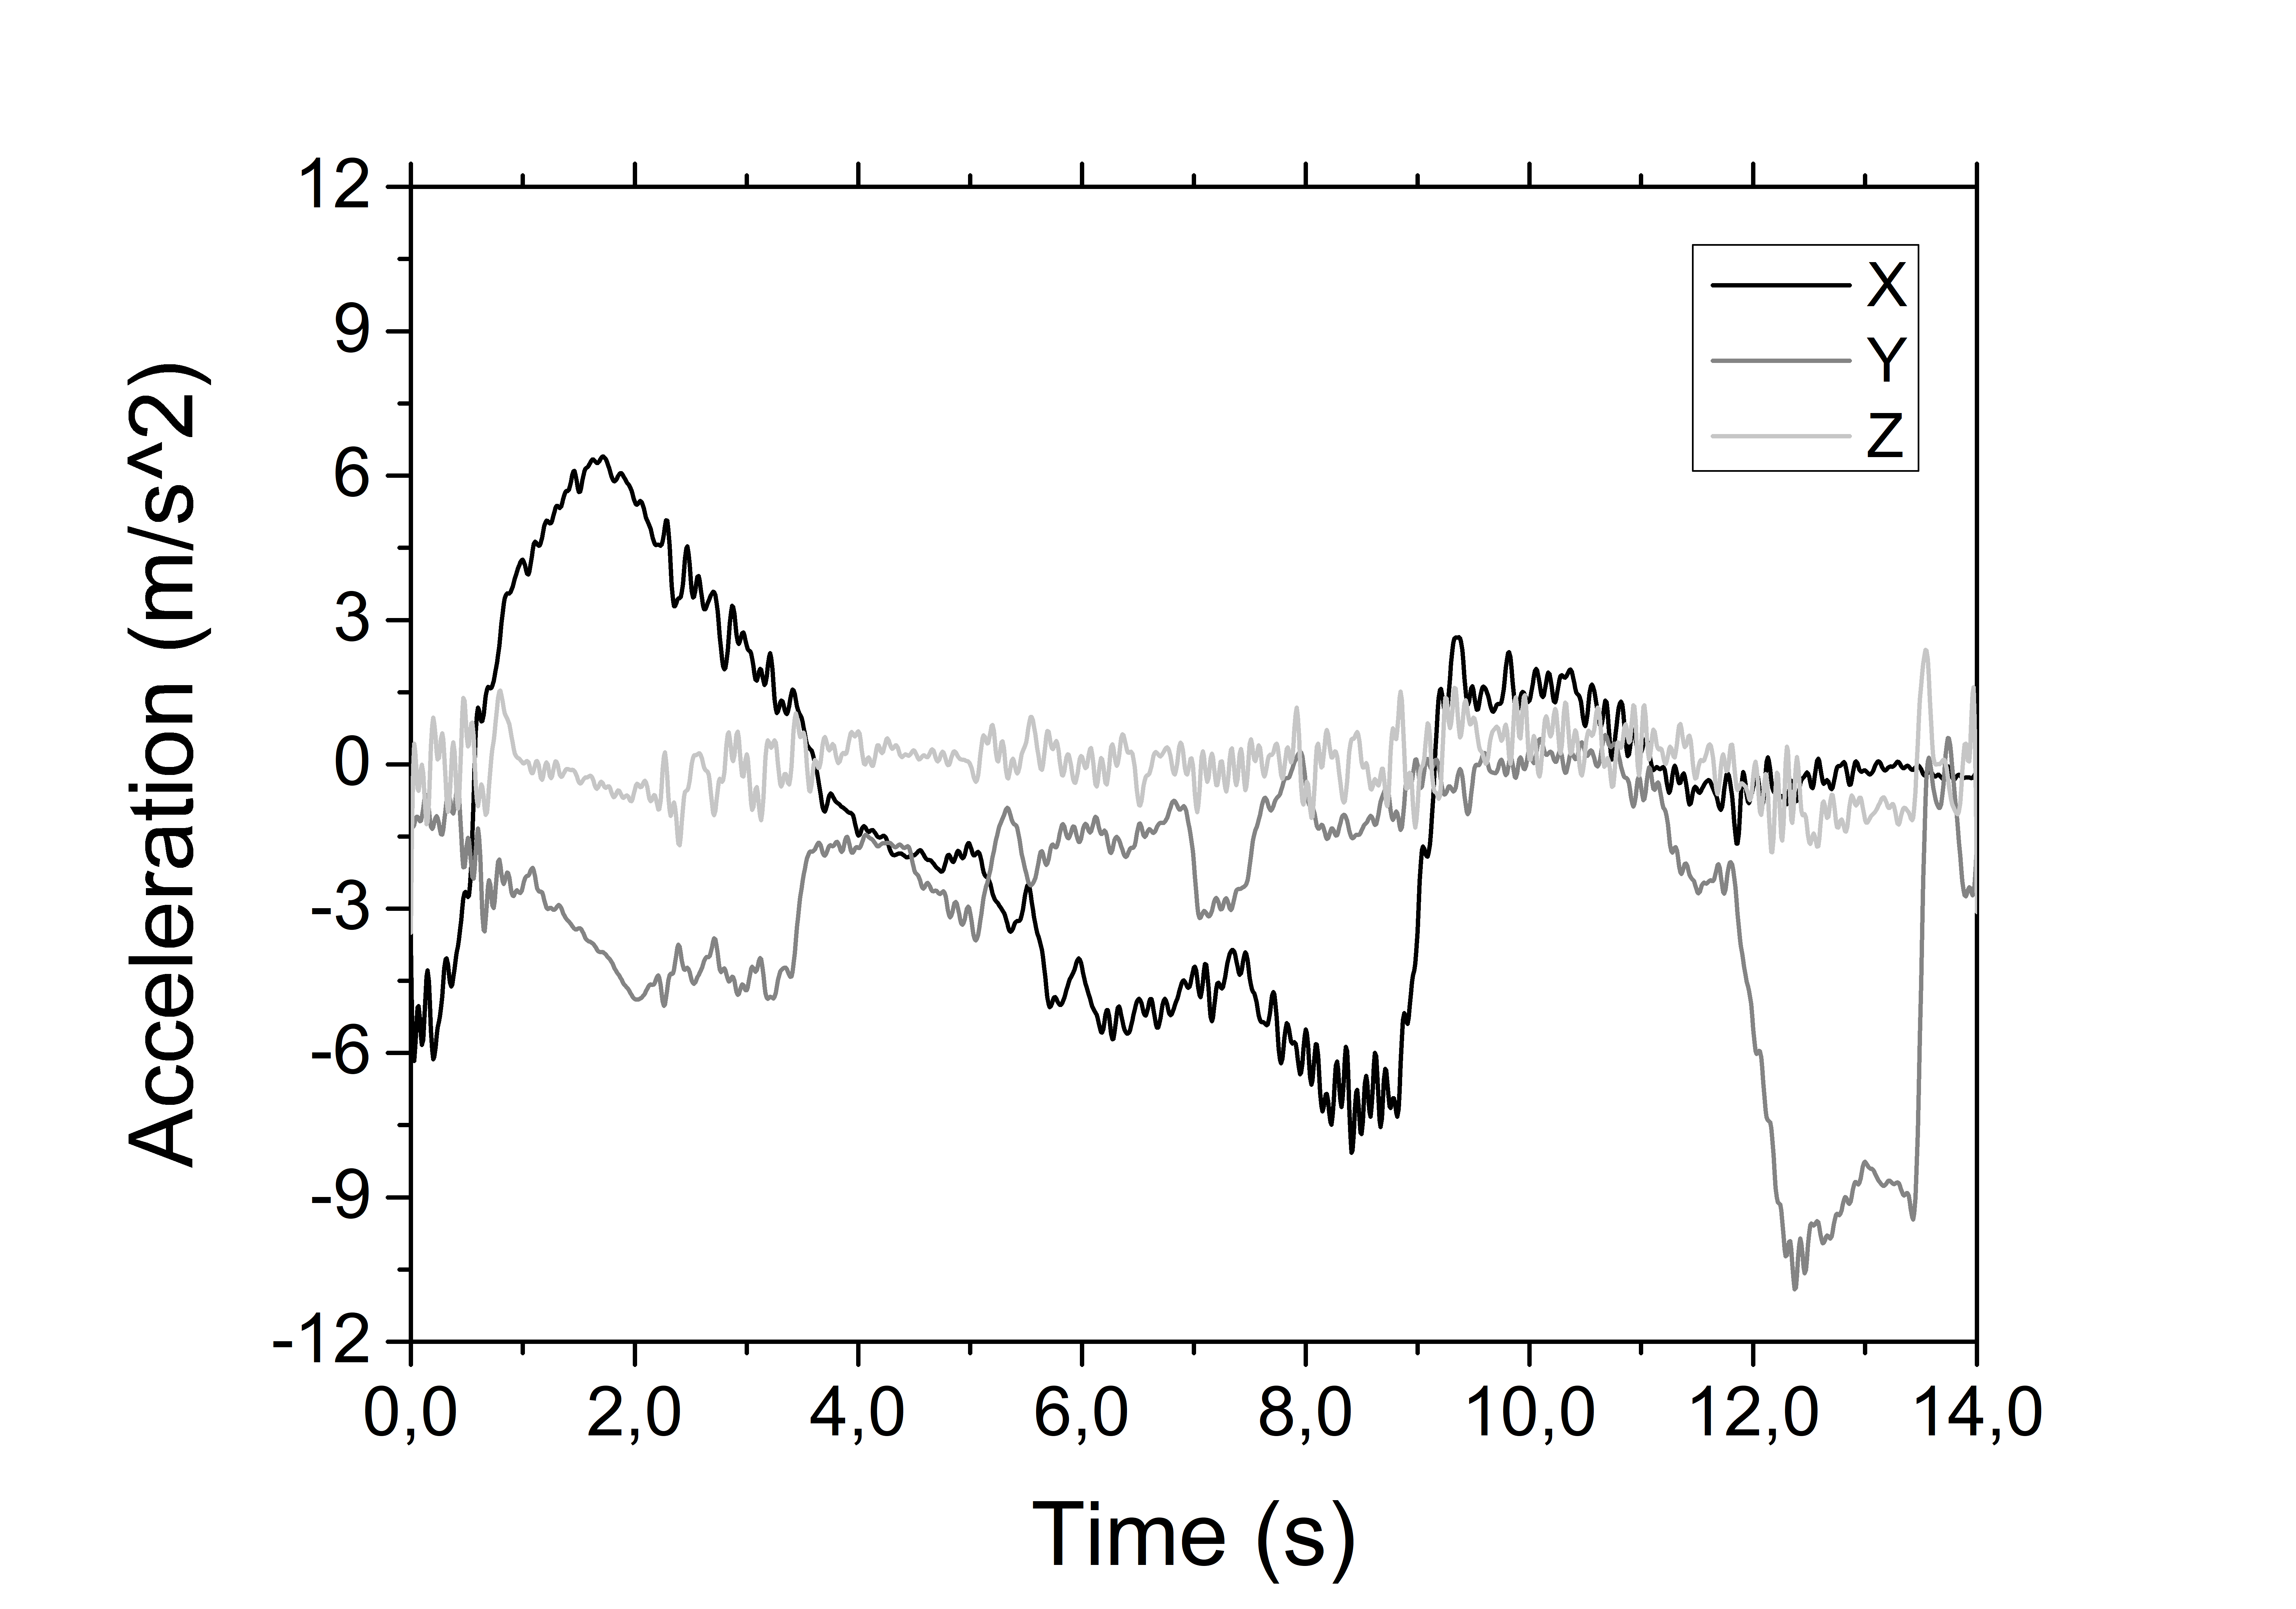
\includegraphics[width=6cm]{Images/Acceleration}
\end{figure}

\begin{figure}[h!]
	\centering
	\includegraphics[width=6cm]{Images/FFTStationary}
\end{figure}

\section{Project Parameters}
In order to choose the right parameters to implement in the driving simulator it was decided to start from two different models of already developed structure for driving simulation.\\
The first one is the Advanced VehicleDriving Simulator (aVDS) developed by ABDynamics (that is the structure on which this project is mainly based). Moreover, in order to obtain more data and to make a comparison with other systems usually exploited in this field, it was analysed the parameters of the 6DOF Motion System designed by CKAS Mechatronics.\\
After that, focusing on the decision of checking if the design parameters given by the catalogues were actually correlated to a real behaviour of a car, it was decided to take some experimental data. In order to do this, it was taken a common car and exploiting the functionalities of the MATLAB application available for smartphones, it was collected some data as: linear acceleration (along the three Cartesian axes), orientation ( Roll, Pitch and Yaw) and angular velocity (along the three Cartesian axes). Furthermore, making some specific maneuvers as narrow curves and rapid acceleration and strong breaking performed both separated and together in order to see different results.\\
At the end, these experimental data were elaborated in MATLAB and then, merging both the parameters from the catalogues and the experimental ones, two final tables were created. Table \ref{t:SystemRequirements1} and Table \ref{t:SystemRequirements2} collect the parameters that will be used for the development of this project. 

\begin{table}[h]
\centering
\begin{tabular}{C{0.5cm}C{1.3cm}C{1.3cm}C{1.3cm}}
	& \textbf{Yaw} & \textbf{Pitch} & \textbf{Roll} \\
	\hline
	\hline
	\\
	\textbf{P} & \( \pm 30 \) & \( \pm 15 \) & \( \pm 30 \) \\
	\textbf{V} & \( \pm 23 \) & \( \pm 23 \) & \( \pm 23 \) \\
	\textbf{A} & \( \pm 150 \) & \( \pm 150 \) & \( \pm 150 \) \\
	\textbf{B} & \( 35 \) & \( 50 \) & \( 35 \) \\
	\\
	\hline
\end{tabular}
\caption{Angular system requirements. \textbf{P} = limitations [\( ^\circ \)], \textbf{V} = velocity [\( ^\circ/s \)], \textbf{A} = acceleration [\( ^\circ/s^2 \)] and \textbf{B} = bandwidth [\( Hz \)].}
\label{t:SystemRequirements1}
\end{table}
\begin{table}[h]
\centering
\begin{tabular}{C{0.5cm}C{1.3cm}C{1.3cm}C{1.3cm}}
	& \textbf{Surge} & \textbf{Sway} & \textbf{Heave}\\
	\hline
	\hline
	\vspace{0.05cm}\textbf{P} & \vspace{0.05cm}\( \pm 65 \) & \vspace{0.05cm}\( \pm 65 \) & \vspace{0.05cm}\( \pm 65 \) \\
	\textbf{V} & \( \pm 100 \) & \( \pm 100 \) & \( \pm 100 \) \\
	\textbf{A} & \( \pm 13.2 \) & \( \pm 9.5 \) & \( \pm 13.4 \) \\
	\textbf{B} & \( 15 \) & \( 35 \) & \( 35 \)
	\vspace{0.15cm} \\
	\hline
\end{tabular}
\caption{Dimensional system requirements. \textbf{P} = limitations [\( mm \)], \textbf{V} = velocity [\( mm/s \)], \textbf{A} = acceleration [\( m/s^2 \)] and \textbf{B} = bandwidth [\( Hz \)].}
\label{t:SystemRequirements2}
\end{table}
\section{Indexes}
Starting from the above mentioned parameters, performance indexes have been identified and divided in three main groups. To each of them, a priority coefficient (P) has been assigned.
\\The general reasoning behind the definition of the kinematic indexes is based on the hypothesis that a good and uniform behaviour in the correlation between engineering parameters has a bigger impact on the performance of the system than the parameters themselves seen as stand alone. The kinematics objectives are:
\begin{itemize}
	\item optimization of Sway - Yaw, Sway - Roll, and Surge - Pitch workspaces | P = 10;
	\item small error between desired and actual parameters regarding pose of the platform and its velocity | P = 7;
	\item small changes of output variables (platform) after big changes in the input ones (actuator) | P = 5;
	\item small ratio between lateral 1D workspace and envelope | P = 4.
\end{itemize}
The most important dynamics indexes correlates kinematic variables (angles) of the platform with their second derivative. The aim is to obtain:
\begin{itemize}
	\item uniform dynamic behaviour in each zone of the workspace, for each plane. This means optimization of the workspaces between Roll and Pitch angles and their second derivatives | P = 10;
	\item small error between desired and actual values of maximum angular and linear acceleration | P = 7.
\end{itemize}
Cross planes requirements have not been assigned in this initial stage.
\\ The identification of the control indexes is based on the hypothesis that low frequency dynamics - with high amplitude - requires absence of overshoot, accepting a loss in the rapidity to convergence to the desired state, so that the user's feel is realistic. On the other side, high frequency dynamics - with low amplitude - should involve rapid convergence to the desired state, accepting a certain value of overshoot. This approach, in first hypothesis, should not compromise the user experience.

\begin{thebibliography}{}
\bibitem{aVDS}
\Virgolette{\textit{Advanced Vehicle Driving Simulator}}, \textsc{ABDynamics}.

\bibitem{CKAS}
\Virgolette{\textit{6DOF Motion System}}, \textsc{CKAS}.

\bibitem{Kasim}
M. Kasim A. J., \Virgolette{\textit{Design and development of 6-dof motion platform for vehicle driving simulator}}, Universiti Teknologi Malaysia.
\end{thebibliography}
\end{document}
